\documentclass[a4j]{jarticle}

\usepackage{jsaisig}
\usepackage[dvipdfmx]{graphicx}
\usepackage{booktabs}
\usepackage{multirow}
\usepackage{url}
\usepackage[dvipdfmx,hidelinks]{hyperref}
\usepackage[absolute,overlay]{textpos}
\setlength{\TPHorizModule}{1mm}
\setlength{\TPVertModule}{1mm}

\input{email}
% Auto-generated by scripts/analyze.py. DO NOT EDIT.
% Reference macros with trailing {} in body text to preserve spacing:
%   e.g. \bestModel{} で ... , \nModels{} 種のモデル

% ==== Experiment scale ====
\newcommand{\nModels}{12}
\newcommand{\nConfigs}{4}
\newcommand{\nItems}{30}
\newcommand{\nCombos}{1440}
\newcommand{\nVendors}{3}
\newcommand{\totalSpend}{\$79.79}

% ==== Bootstrap 95% CI for best combo ====
\newcommand{\bestCIlo}{0.746}
\newcommand{\bestCIhi}{0.903}

% ==== Bootstrap 95% CI for best Single combo ====
\newcommand{\bestSingleModel}{Opus 5}
\newcommand{\bestSingleFtwo}{0.738}
\newcommand{\bestSingleCIlo}{0.645}
\newcommand{\bestSingleCIhi}{0.848}

% ==== Best F2 combo ====
\newcommand{\bestModel}{GPT-5 mini}
\newcommand{\bestConfig}{Multi-run}
\newcommand{\bestFtwo}{0.826}
\newcommand{\bestCost}{\$0.0206}

% ==== Cost spread ====
\newcommand{\cheapestCost}{\$0.0005}
\newcommand{\priciestCost}{\$0.2182}
\newcommand{\costSpread}{415}

% ==== Per-model best-config wins ====
\newcommand{\modelMultiWins}{8}
\newcommand{\modelAdvWins}{0}
\newcommand{\modelSingleWins}{2}
\newcommand{\modelParWins}{2}

% ==== Per-config mean F2 / cost ====
\newcommand{\singleMeanF}{0.536}
\newcommand{\singleMeanCost}{\$0.0196}
\newcommand{\parallelMeanF}{0.514}
\newcommand{\parallelMeanCost}{\$0.0628}
\newcommand{\adversarialMeanF}{0.479}
\newcommand{\adversarialMeanCost}{\$0.0453}
\newcommand{\multiMeanF}{0.602}
\newcommand{\multiMeanCost}{\$0.0939}

% ==== Pareto-dominated models ====
\newcommand{\dominatedModels}{Sonnet 5，GPT-5，Opus 5，Fable 5，GPT-5.6 luna，GPT-5.6 terra，o3，Gemini 3.6 flash，Gemini 3.1 pro-preview}
\newcommand{\dominatedCount}{9}

% ==== Per-repo (language) best (model / config) ====
\newcommand{\bestByFastapi}{GPT-5 mini / Multi-run}
\newcommand{\bestByFastapiF}{0.722}
\newcommand{\bestByValibot}{GPT-5 mini / Multi-run}
\newcommand{\bestByValibotF}{0.777}
\newcommand{\bestByChi}{GPT-5 mini / Multi-run}
\newcommand{\bestByChiF}{0.972}
\newcommand{\bestByPgrust}{GPT-5 mini / Multi-run}
\newcommand{\bestByPgrustF}{0.909}

% ==== Category breakdown ====
\newcommand{\nCategories}{8}
\newcommand{\catWinners}{GPT-5 mini (5 種別)，Haiku 4.5 (3 種別)}
\newcommand{\perfectCats}{other・type-safety・api-misuse・error-handling}
\newcommand{\perfectCount}{4}
\newcommand{\hardestCat}{concurrency}
\newcommand{\hardestBestFtwo}{0.667}
\newcommand{\catNmin}{1}
\newcommand{\catNmax}{15}



\setlength{\intextsep}{6pt}
\setlength{\textfloatsep}{8pt}
\setlength{\floatsep}{6pt}

\begin{document}

\title{AI コードレビュー・オーケストレーション構成のコスト-欠陥検出性能比較}

\etitle{Cost-vs-Defect Detection Performance Comparison of AI Code Review Orchestration Configurations}

\author{高原 大明\afil{1}%
\thanks{連絡先: 北陸先端科学技術大学院大学 \newline%
E-mail: \authorEmail}\quad%
岡田 将吾\afil{1}\quad%
伊集院 幸輝\afil{1}\\
Hiroaki Takahara\afil{1} \quad Shogo Okada\afil{1} \quad Koki Ijuin\afil{1}}

\affiliation{%
\afil{1} 北陸先端科学技術大学院大学\\
\afil{1} Japan Advanced Institute of Science and Technology}

\abstract{%
Aspect-parallel review, adversarial critique, and multi-run
aggregation extend LLM code review beyond single-reviewer setups.
Prior evaluations do not control compute budget, so we cannot tell
whether these constructions add anything the raw compute would not.
We build a defect-detection benchmark by inverting real bug-fix
commits from four single-language open-source (OSS) repositories
(Python, TypeScript, Go, Rust). One repository postdates current
model cutoffs, giving a leakage-free control. Across \nItems{} items,
\nModels{} models, \nVendors{} vendors, and 4 orchestrations, we
rank by $F_2$ (Recall weighted 4$\times$ over Precision to match
the asymmetric cost of missed defects). \dominatedCount{} of
\nModels{} models (none of their 4 configurations enters the front)
fall off the cost-$F_2$ Pareto front. Multi-run aggregation
wins in \modelMultiWins{} of \nModels{} models and every one of
the four repositories. Across cost bands, cheap models running
Multi-run beat premium single-shot selection above \$0.01/item;
returns flatten above \$0.05.
}

\maketitle
\thispagestyle{empty}
\begin{textblock*}{60mm}(140mm,15mm)
\raggedleft\small
人工知能学会第二種研究会資料\\
汎用人工知能研究会\\
SIG-AGI-033-07
\end{textblock*}

\section{はじめに}

汎用人工知能 (AGI; Artificial General Intelligence) の実現には，多様な課題に対して限られた計算資源の下で柔軟かつ効率的に推論を行う能力が求められる．
近年，大規模言語モデル (LLM) はソフトウェア開発をはじめとする幅広い知的タスクで利用されており，コードレビューの自動化も研究・商用の両面で普及が進んでいる．
LLM を用いたコードレビューの手法として，単一レビュアで全観点を確認する構成が広く使われてきた．
近年はさらに，観点別並列 (Parallel)，反証型構成 (Adversarial)，反復実行集約 (Multi-run) などオーケストレーション構成の提案が続いている\cite{codeagent}．
しかし，これらの構成の優位性を報告する評価の多くは計算量 (トークン消費) を統制しておらず，観測された性能差が構成の構造に由来するのか，単なる計算量増加に由来するのかは切り分けられない．
一般推論ドメインでは，予算を揃えると multi-agent debate 等の優位が消失・逆転するとの報告が複数ある\cite{mad}．
一方，コードレビューでは AI の誤指摘はレビュアが却下すれば対処できるのに対し，見逃しの発見には人手コードレビューを要する．この非対称性の下で上記の知見が成立するかは未検証である．

本研究は次の 3 つの研究課題を設定する．
\begin{itemize}
\setlength{\itemsep}{2pt}
\item \textbf{RQ1}: 同等コスト水準で見たとき，オーケストレーション構成の間に欠陥検出率・偽陽性率の差があるか．
\item \textbf{RQ2}: 観点別並列構成の優位性 (があるとすれば) は，同等コストの Multi-run 集約 (純粋な計算量増加) と比較しても残るか．
\item \textbf{RQ3}: 欠陥の種別によって有利な構成は異なるか．
\end{itemize}

本稿の貢献は次の 3 点である．
\begin{itemize}
\setlength{\itemsep}{2pt}
\item 実オープンソースソフトウェア (以下 OSS) のバグ修正コミット逆適用による，計算予算を統制できる欠陥検出ベンチマークの構築 (\S 3)．
\item \nModels{} モデル $\times$ \nConfigs{} 構成 $\times$ \nItems{} 件のグリッドで得た (コスト, $F_2$) の実測 (\S 4-5)．
\item 予算帯に依存する構成の優劣関係を示すパレートフロントの提示 (\S 5)．
\end{itemize}

\section{関連研究}

\textbf{Multi-agent コードレビュー．}
役割分担型のレビューエージェント\cite{codeagent}をはじめ，LLM multi-agent 構成による欠陥検出の提案は多く，分野の整理は近年の survey\cite{guo2024largelanguagemodelbased}が詳しい．
これら既存研究は個別構成の効果を報告するが，コスト-性能面で複数構成を横断比較したものは調査の範囲では存在しない．
一方，商用レビューエージェントの実証評価では，多数のツールで指摘のシグナル比が低くノイズ過多であることが報告されており，適合率を含めて評価する必要がある．

\textbf{計算量統制下の multi-agent 評価．}
一般推論タスクでは，multi-agent debate\cite{mad}や self-refinement\cite{reflexion}の性能向上が，同一計算量の単純な多数決や複数候補からの最良選択と比較すると消失するとの報告がある．
Wang らは強い prompt を与えた single-agent が multi-agent 議論のほぼ最良と同等となることを実証し，multi-agent 優位の境界を再考している\cite{wang2024rethinkingboundsllmreasoning}．
コードレビュードメインでこの統制比較を行った研究は，調査の範囲では存在しない．

\textbf{欠陥ベンチマーク．}
Defects4J\cite{defects4j}や SWE-bench\cite{swebench}など実バグ由来のベンチマークが広く使われているが，いずれも修正パッチ生成の評価が主目的であり，レビュー (差分に対する指摘) の評価を目的とした，計算予算を統制できる形式のベンチマークは整備されていない (ソフトウェア工学 (software engineering; SE) における LLM 応用の広範な整理は\cite{zhang2024surveylargelanguagemodels}を参照)．
また，これら既知ベンチマークは LLM の学習データに含まれる可能性が高く，暗記による性能の過大評価 (leakage) が指摘されている．

\section{ベンチマーク構築}

\subsection{設計方針}

実 OSS のバグ修正コミット $F$ を逆適用し，「バグを含む変更を提出する pull request (以下 PR)」を合成する．
基底状態を $F$ 適用後の正常コードとし，$F^{-1}$ をレビュー対象の差分として提示する．
たとえば fix コミットが境界チェック \verb|if (x < 0) return -1;| を追加していた場合，逆適用ではこの行を削除した差分を PR として提示し，レビュアがこの見落としを指摘できるかを評価する．
これにより全リポジトリ・全バグに一律の手続きを適用でき，正解 (ground truth) も fix の変更箇所として一意に定義される．
合成 PR であって実在した PR ではない点は本手法の限界であり，\ref{sec:limitations} 節で議論する．

\subsection{対象リポジトリ}

表\ref{tab:repos}の 4 リポジトリを対象とする．
リポジトリ効果と言語効果を分離するため，各リポジトリが単一言語で構成されるものを選定し，言語 (Python, TypeScript, Go, Rust) とドメイン (Web フレームワーク, スキーマ検証, HTTP ルータ, データベースエンジン) を分散させた．
また既存ベンチマーク (SWE-bench 等) との重複がないことを確認し，leakage リスクを下げた．

pgrust は PostgreSQL の Rust 移植であり，全履歴が 2026 年 6 月以降，すなわち本稿対象モデルの知識カットオフ後に作られた AI 支援開発リポジトリである．
このため本稿対象モデルに対する leakage リスクを大幅に低減できる統制群として機能し，AI 支援下で作成されたコードを対象とするレビュー課題を含む．
さらに PostgreSQL の回帰テスト群 (46,000 クエリ超) を欠陥実在性の判定基準として利用できる．
一方で単独作者・AI 支援によるバグ分布の偏りは \ref{sec:limitations} 節で明記する．

\begin{table}[!t]
 \centering
 \caption{対象リポジトリ．}
 \label{tab:repos}
 \footnotesize
 \setlength{\tabcolsep}{4pt}
 \begin{tabular}{llll}
  \toprule
  リポジトリ & 言語 & ドメイン & ライセンス \\
  \midrule
  fastapi & Python & Web FW & MIT \\
  valibot & TypeScript & Schema検証 & MIT \\
  chi & Go & HTTP ルータ & MIT \\
  pgrust & Rust & DB エンジン & AGPL-3.0 \\
  \bottomrule
 \end{tabular}
\end{table}

\footnotetext[1]{%
\scriptsize
fastapi: \url{https://github.com/fastapi/fastapi} commit \href{https://github.com/fastapi/fastapi/commit/afe4112}{\texttt{afe4112}};\quad
valibot: \url{https://github.com/open-circle/valibot} commit \href{https://github.com/open-circle/valibot/commit/32247b3}{\texttt{32247b3}};\quad
chi: \url{https://github.com/go-chi/chi} commit \href{https://github.com/go-chi/chi/commit/8b258c7}{\texttt{8b258c7}};\quad
pgrust: \url{https://github.com/malisper/pgrust} commit \href{https://github.com/malisper/pgrust/commit/c9aecbd}{\texttt{c9aecbd}}．%
}
\addtocounter{footnote}{1}

\subsection{構築パイプライン}

構築は 4 段階からなる．
各段階の生成物は JSON としてリポジトリ\footnote{\url{https://github.com/hiroaki222/review-orchestration-bench}}で公開している．

\textbf{(1) 抽出．}
リポジトリごとの commit 規約に合わせた正規表現で bug fix 候補コミットを抽出した (計 1,544 件)．

\textbf{(2) 機械フィルタ．}
非テストコードの変更が 100 行以下かつ 5 ファイル以下，docs・typo・revert 等を除外する条件で 816 件に絞った．
行数はテストコードを除いて数える (1 行の修正に大規模なテストが付随するケースを誤って除外しないため)．

\textbf{(3) LLM 分類と懐疑的再検証．}
API コスト削減のため 816 件全数投入は避け，post-cutoff 全数と目標未達リポジトリの pre-cutoff 補充を反復投入して累計 201 件を分類した．
LLM エージェントに各候補の diff を読ませ，実挙動バグの修正であるか (機能追加・リファクタ・移植作業の補完等を除外)，逆適用が自然なレビュー課題となるか，バグ種別，深刻度を判定した．
バッチ間で LLM の判定基準は一貫せず，判定が極端なバッチには反証プロンプトの再検証エージェントを適用し，4 件の判定を反転させた．
最終的に 201 件中 135 件が逆適用可能 (真のバグ修正かつ逆適用が自然) と判定された (目標 85 件に対して $\sim 1.6\times$ の余裕)．
分類は Claude 系 (Sonnet 5) で行い，異系統 LLM (Codex/GPT 系) による 17 件 (repo 比例層別) の独立再判定で 12 件一致を確認した．LLM 分類に由来する選定バイアスの議論は \ref{sec:limitations} 節に譲る．

\textbf{(4) 層別サンプリング．}
乱数を用いない決定的アルゴリズム (知識カットオフ後のコミットを優先し，残りをバグ種別のラウンドロビンで補充) により，85 件 (fastapi 25 / valibot 20 / chi 15 / pgrust 25) を選定した．
内訳はカットオフ後 49 件・カットオフ前 36 件であり，種別は logic (論理誤り) 34，type-safety (型安全性) 15，error-handling (例外処理) 10，concurrency (並行性) 7，security (セキュリティ) 6，その他 13 である．

\subsection{Leakage 統制}

境界日を 2026-01-01 に設定し，以降のコミットを post-cutoff として優先採用，不足分は pre-cutoff から補充した上で，前後の別を共変量として分析に組み込む．
この境界は主要モデルのカットオフのうち下限に近い日付を選び，全モデルで知識カットオフ後とみなせる範囲を最大化した．モデルごとの真のカットオフは異なるため厳密には近似だが，pgrust は全履歴が 2026-06 以降のため全モデル共通のカットオフ後データとなる．
事前調査では，post-cutoff のみで必要数を確保できるリポジトリは pgrust のみであり (他 3 リポジトリの post-cutoff における逆適用可能件数は 4〜11 件)，時期混合と共変量統制は必須であった．

\section{実験設計}

構築したベンチマークから \nItems{} 件を層別抽出し，次の \nConfigs{} 構成 $\times$ \nModels{} モデル $\times$ \nItems{} 件のグリッドで欠陥検出性能とコストを実測した．
括弧内の数字は LLM 呼び出し回数を表す．
\begin{itemize}
\setlength{\itemsep}{2pt}
\item \textbf{Single}: 単一レビュアが全観点を担当 (1 回)．
\item \textbf{Parallel}: 4 観点 (correctness, concurrency, api-misuse, security) を独立実行し和集合を取得 (4 回)．
\item \textbf{Adversarial}: レビュアが指摘を生成する初回 1 回の後，各指摘に反証プロンプトを 2 回適用し半数以上の支持で採用する (指摘数 $k$ に対し $1+2k$ 回)．
\item \textbf{Multi-run}: 同一プロンプトを 5 回実行し 2 票以上の指摘のみ採用する計算量統制の対照群 (5 回)．
\end{itemize}

全構成でシステムプロンプトは共通の基底 \textit{``You are a senior software engineer reviewing a pull request for defects the change would introduce (not stylistic nitpicks).''} を用い，各指摘を \texttt{\{file, line\_start, line\_end, severity, category, summary\}} の JSON 配列として出力させる．
Parallel では 4 観点 (correctness, concurrency, api-misuse, security) それぞれに焦点範囲を絞る補助文を前置し，Adversarial の反証プロンプトは \textit{``Default to REFUTED unless the diff clearly demonstrates the bug.''} を用いる．
Multi-run は Single と同一プロンプトを 5 回反復する．
完全な文言は公開リポジトリの \href{https://github.com/hiroaki222/review-orchestration-bench/blob/main/src/harness/prompts.py}{\texttt{src/harness/prompts.py}} を参照．

モデルは Anthropic (Haiku 4.5, Sonnet 5, Opus 5, Fable 5)，OpenAI (GPT-5 mini, GPT-5, GPT-5.6 luna, GPT-5.6 terra, o3)，Google (Gemini 3.5 flash-lite, 3.6 flash, 3.1 pro-preview) の \nVendors{} ベンダ \nModels{} モデルを対象とし，各ベンダで廉価モデルから高性能モデルまでの価格帯を横断させた．
検出判定は指摘の (file, line 範囲) と ground truth のハンク範囲の重なり (許容 $\pm 2$ 行) を機械判定する．
主指標には $F_2$ スコア ($\beta = 2$, $F_2 = 5PR / (4P + R)$) を採用する．これは再現率 (Recall; 真のバグを取りこぼさない度合い) を適合率 (Precision; 指摘が本物である割合) の 4 倍重視する指標である．コードレビュー実務において，AI が挙げた候補の却下はレビュアの確認で対処できるが，AI が見逃したバグの発見は最終的に人手コードレビューを要する．前者に比べ後者の対応工数が高いため，見逃しを減らすことを優先する $F_2$ を主指標に据えた．参考として適合率と再現率も併記する．

\section{結果}

\nItems{} 件 $\times$ \nModels{} モデル $\times$ \nConfigs{} 構成 $=$ \nCombos{} 件の結果を表\ref{tab:main}に示す (パレートフロント 6 点は $^{P}$ で明示)．コスト・$F_2$ 散布は図\ref{fig:pareto}に示す．

\begin{table}[!t]
  \centering
  \caption{構成別の検出性能とコスト (各セル 30 件平均，$N=30$)．太字はモデル内最高 $F_2$，下線付き太字は全体最高，$^{P}$ はパレートフロント (図\ref{fig:pareto}と対応)．略号: Sin = Single, Par = Parallel, Adv = Adversarial, MR = Multi-run．}
  \label{tab:main}
  \scriptsize
  \setlength{\tabcolsep}{2pt}
  \resizebox{\linewidth}{!}{\begin{tabular}{@{}llrrrr@{}}
\toprule
Model & Cfg & Prec & Rec & $F_2$ & \$/item \\
\midrule
\multicolumn{6}{@{}l}{\textit{Anthropic}} \\[1pt]
\multirow[t]{4}{*}{Haiku 4.5} & Sin & 0.80 & 0.60 & 0.635$^{P}$ & 0.0019 \\
 & Par & 0.25 & 0.68 & 0.503 & 0.0076 \\
 & Adv & 0.86 & 0.47 & 0.518 & 0.0066 \\
 & MR & 0.79 & 0.65 & \textbf{0.671}$^{P}$ & 0.0096 \\
\addlinespace[2pt]
\multirow[t]{4}{*}{Sonnet 5} & Sin & 0.88 & 0.51 & 0.561 & 0.0091 \\
 & Par & 0.33 & 0.62 & 0.526 & 0.0276 \\
 & Adv & 0.90 & 0.38 & 0.432 & 0.0204 \\
 & MR & 0.81 & 0.57 & \textbf{0.609} & 0.0402 \\
\addlinespace[2pt]
\multirow[t]{4}{*}{Opus 5} & Sin & 0.82 & 0.72 & \textbf{0.738} & 0.0341 \\
 & Par & 0.25 & 0.74 & 0.533 & 0.1215 \\
 & Adv & 0.84 & 0.53 & 0.571 & 0.1243 \\
 & MR & 0.80 & 0.72 & 0.736 & 0.1755 \\
\addlinespace[2pt]
\multirow[t]{4}{*}{Fable 5} & Sin & 0.70 & 0.56 & 0.583 & 0.0584 \\
 & Par & 0.29 & 0.62 & 0.502 & 0.1747 \\
 & Adv & 0.85 & 0.41 & 0.459 & 0.1461 \\
 & MR & 0.85 & 0.59 & \textbf{0.627} & 0.2182 \\
\midrule
\multicolumn{6}{@{}l}{\textit{OpenAI}} \\[1pt]
\multirow[t]{4}{*}{GPT-5 mini} & Sin & 0.59 & 0.29 & 0.327 & 0.0035 \\
 & Par & 0.25 & 0.68 & 0.503 & 0.0143 \\
 & Adv & 0.74 & 0.74 & 0.735$^{P}$ & 0.0102 \\
 & MR & 0.84 & 0.82 & \underline{\textbf{0.826}}$^{P}$ & 0.0206 \\
\addlinespace[2pt]
\multirow[t]{4}{*}{GPT-5} & Sin & 0.88 & 0.53 & \textbf{0.575} & 0.0341 \\
 & Par & 0.36 & 0.57 & 0.513 & 0.1036 \\
 & Adv & 0.91 & 0.43 & 0.477 & 0.0682 \\
 & MR & 0.65 & 0.53 & 0.550 & 0.1794 \\
\addlinespace[2pt]
\multirow[t]{4}{*}{GPT-5.6 luna} & Sin & 0.97 & 0.49 & 0.539 & 0.0067 \\
 & Par & 0.38 & 0.57 & 0.521 & 0.0234 \\
 & Adv & 0.91 & 0.44 & 0.492 & 0.0119 \\
 & MR & 0.82 & 0.53 & \textbf{0.570} & 0.0378 \\
\addlinespace[2pt]
\multirow[t]{4}{*}{GPT-5.6 terra} & Sin & 0.97 & 0.50 & 0.554 & 0.0161 \\
 & Par & 0.33 & 0.54 & 0.482 & 0.0464 \\
 & Adv & 0.97 & 0.44 & 0.495 & 0.0238 \\
 & MR & 0.86 & 0.54 & \textbf{0.587} & 0.0796 \\
\addlinespace[2pt]
\multirow[t]{4}{*}{o3} & Sin & 0.94 & 0.47 & 0.523 & 0.0153 \\
 & Par & 0.33 & 0.63 & 0.532 & 0.0487 \\
 & Adv & 0.95 & 0.29 & 0.341 & 0.0357 \\
 & MR & 0.86 & 0.56 & \textbf{0.601} & 0.0728 \\
\midrule
\multicolumn{6}{@{}l}{\textit{Google}} \\[1pt]
\multirow[t]{4}{*}{Gemini 3.5 flash-lite} & Sin & 0.96 & 0.38 & 0.435$^{P}$ & 0.0005 \\
 & Par & 0.45 & 0.53 & \textbf{0.511}$^{P}$ & 0.0019 \\
 & Adv & 0.94 & 0.24 & 0.277 & 0.0011 \\
 & MR & 0.88 & 0.34 & 0.386 & 0.0024 \\
\addlinespace[2pt]
\multirow[t]{4}{*}{Gemini 3.6 flash} & Sin & 0.93 & 0.40 & 0.449 & 0.0224 \\
 & Par & 0.44 & 0.53 & 0.510 & 0.0650 \\
 & Adv & 0.93 & 0.40 & 0.449 & 0.0364 \\
 & MR & 0.89 & 0.50 & \textbf{0.548} & 0.1090 \\
\addlinespace[2pt]
\multirow[t]{4}{*}{Gemini 3.1 pro-preview} & Sin & 0.86 & 0.47 & 0.518 & 0.0331 \\
 & Par & 0.36 & 0.60 & \textbf{0.532} & 0.1191 \\
 & Adv & 0.94 & 0.46 & 0.508 & 0.0595 \\
 & MR & 0.86 & 0.47 & 0.518 & 0.1811 \\
\midrule
\multicolumn{6}{@{}l}{\textit{Mean $F_2$ over models}: Sin\,0.536 / Par\,0.514 / Adv\,0.479 / MR\,\textbf{0.602}} \\
\bottomrule
\end{tabular}
}
\end{table}

\bestModel{} の \bestConfig{} 構成が最良で $F_2 = \bestFtwo{}$，項目あたり平均 \bestCost{} を要した．
項目あたりコストは最安 \cheapestCost{} から最高 \priciestCost{} まで \costSpread{} 倍の広がりを持つが，$F_2$ はコストに単調ではない．
構成別平均 $F_2$ は Multi-run が \multiMeanF{} と最も高く，続いて Single \singleMeanF{}，Parallel \parallelMeanF{}，Adversarial \adversarialMeanF{} となる．
再現率重視の $F_2$ では，Adversarial の反証プロンプトが誤検出を減らして適合率を上げる一方で本物のバグまで却下し再現率を下げるため，総合では Single を下回る．Multi-run の反復実行集約 (2/5 しきい値) は適合率と再現率の双方を伸ばし他構成を上回った．
モデル別に最良 $F_2$ の構成を集計すると，\nModels{} モデル中 \modelMultiWins{} で Multi-run が最良となり (表\ref{tab:main})，モデル選択によらず Multi-run 優位の傾向が観察された．本結果は，予算統制下でマルチエージェント議論 (multi-agent debate) や自己改良 (self-refinement) の優位が消失し得るという既報\cite{mad,reflexion,wang2024rethinkingboundsllmreasoning}と整合的である．
Multi-run 優位について，統計的側面と指標感度の 2 面から検証する．最良組 (\bestModel{}/\bestConfig{}, $F_2 = \bestFtwo{}$) の項目 bootstrap 95\% 信頼区間は $[\bestCIlo{}, \bestCIhi{}]$ で，Single 最良 (\bestSingleModel{}, $F_2 = \bestSingleFtwo{}$，信頼区間 $[\bestSingleCIlo{}, \bestSingleCIhi{}]$) と部分的に重なるため，$N=\nItems{}$ の本実験では単一組間の有意差は示せない．一方，モデル別集計では \nModels{} モデル中 \modelMultiWins{} で Multi-run が最良となり，複数モデルで同様の傾向が見られた．$\beta \in \{1, 1.5, 2, 3\}$ で $F_\beta$ を振った感度分析 (表\ref{tab:beta}) でも Multi-run は全帯で最高値を維持する．Adversarial は再現率重み増加で順位を下げ Parallel は上げるため，$\beta = 3$ では Parallel が Single を上回る．

\begin{table}[!t]
  \centering
  \caption{$F_\beta$ の $\beta$ 感度分析 (構成別平均 $F_\beta$)．太字は各 $\beta$ 列の最高値．}
  \label{tab:beta}
  \footnotesize
  \begin{tabular}{@{}lrrrr@{}}
\toprule
Config & $F_{1}$ & $F_{1.5}$ & $F_{2}$ & $F_{3}$ \\
\midrule
Single & 0.619 & 0.563 & 0.536 & 0.514 \\
Parallel & 0.424 & 0.477 & 0.514 & 0.556 \\
Adversarial & 0.572 & 0.508 & 0.479 & 0.456 \\
Multi-run & \textbf{0.665} & \textbf{0.623} & \textbf{0.603} & \textbf{0.585} \\
\bottomrule
\end{tabular}

\end{table}

パレートフロントでは，全構成で他モデルに (コスト, $F_2$) の両面で劣位となりフロントから外れたモデルは \dominatedModels{} である．
Multi-run が単発を上回るのは項目あたり \$0.01 以上の予算帯からで，それ以上では価格帯上位モデルを単純選択するよりも下位モデルに Multi-run を組み合わせる方が支配的な戦略となる．

\begin{figure}[!t]
  \centering
  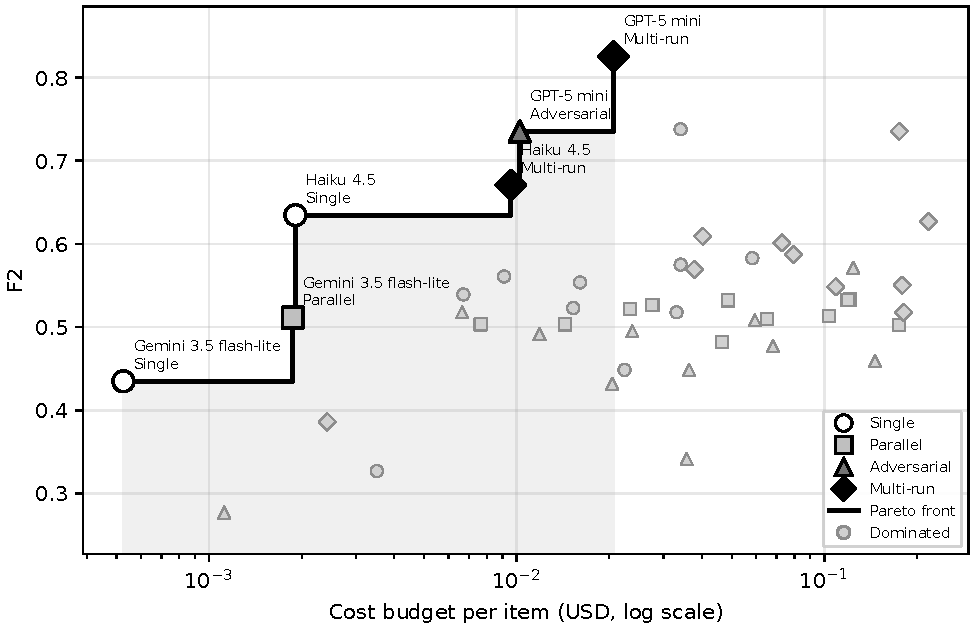
\includegraphics[width=\linewidth]{fig/pareto.pdf}
  \caption{項目あたりコスト (対数軸) と $F_2$ の散布．マーカの形状は構成を表す．パレートフロント上の点は黒縁で強調しモデル名を注記した (表\ref{tab:main} の $^{P}$ セルに対応)．フロントから外れた点はグレーで表示する．}
  \label{fig:pareto}
\end{figure}

予算 \$0.002 では追加呼び出しの費用が支配的となり Single 構成 (Haiku 4.5 / Single) が最も高い性能を示すが，\$0.01 でオーケストレーション構成が Single を上回る．さらに \$0.05 以上では Opus 5 単体を含むすべての Single 構成を GPT-5 mini / Multi-run が上回り，予算を 4 倍に増加させても達成可能な最高 $F_2$ は向上しない (図\ref{fig:budget})．
本実験の総 API 支出は \totalSpend{} である．

\begin{figure}[!t]
  \centering
  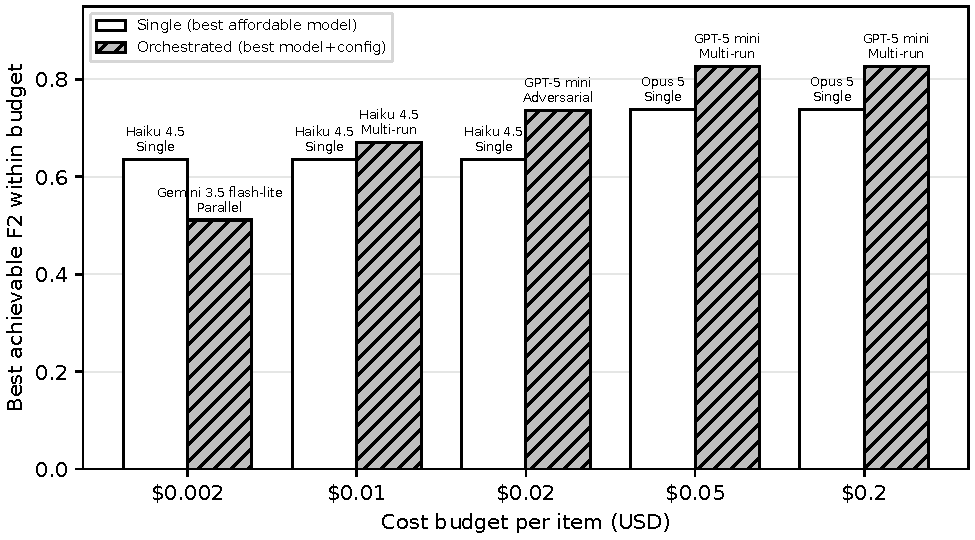
\includegraphics[width=\linewidth]{fig/budget.pdf}
  \caption{項目あたり予算帯ごとの最高 $F_2$ の比較．Single 構成のみで達成可能な最高 $F_2$ と，オーケストレーション構成 (Parallel, Adversarial, Multi-run) で達成可能な最高 $F_2$ を並置する．各棒の上には最高性能を達成したモデル・構成を注記した．}
  \label{fig:budget}
\end{figure}

バグ種別ごとの最高 $F_2$ を表\ref{tab:cat_best}に示す．全 \nCategories{} 種別で最高値を示すのは \catWinners{} であり，種別に応じて最適な (モデル, 構成) が入れ替わる．
種別別最良 $F_2$ は \perfectCats{} の \perfectCount{} 種で 1.000 に達する一方，\hardestCat{} は最良でも \hardestBestFtwo{} と全モデルで相対的に低い値にとどまった．
種別あたりの標本数は \catNmin{}〜\catNmax{} 件と小さく個別順位は暫定的だが，RQ3 に対する予備的示唆として，種別に応じて最適な (モデル, 構成) が入れ替わる可能性が示唆された．

\begin{table}[!t]
  \centering
  \caption{各バグ種別における最高 $F_2$ とそのモデル・構成，および種別あたり項目数 N．$\dagger$ 付き N は小標本 (N $\le$ 2)．}
  \label{tab:cat_best}
  \footnotesize
  \begin{tabular}{@{}lllr@{}}
\toprule
バグ種別 & 最良 (モデル / 構成) & $F_2$ & N \\
\midrule
logic & GPT-5 mini / Multi-run & 0.779 & 15 \\
type-safety & Haiku 4.5 / Single & 1.000 & 2$^{\dagger}$ \\
error-handling & Haiku 4.5 / Multi-run & 1.000 & 1$^{\dagger}$ \\
concurrency & Haiku 4.5 / Adversarial & 0.667 & 3 \\
api-misuse & GPT-5 mini / Multi-run & 1.000 & 4 \\
security & GPT-5 mini / Adversarial & 0.833 & 1$^{\dagger}$ \\
resource-leak & GPT-5 mini / Multi-run & 0.897 & 2$^{\dagger}$ \\
other & GPT-5 mini / Adversarial & 1.000 & 2$^{\dagger}$ \\
\bottomrule
\end{tabular}

\end{table}

言語別の最高 $F_2$ を表\ref{tab:repo_best}に示す．本実験の 4 リポで GPT-5 mini / Multi-run が一貫して最高値を示した．ただし対象は 4 リポに限られる．
一方で達成 $F_2$ は Python \bestByFastapiF{}, TypeScript \bestByValibotF{}, Go \bestByChiF{}, Rust \bestByPgrustF{} の範囲に分布し，タスクの言語・ドメインが検出難度を左右する．

\begin{table}[!t]
  \centering
  \caption{各リポジトリ (言語) における最高 $F_2$ スコアと，そのモデル・構成．}
  \label{tab:repo_best}
  \footnotesize
  \begin{tabular}{@{}lll@{}}
\toprule
リポジトリ (言語) & 最良 (モデル / 構成) & $F_2$ \\
\midrule
Python (fastapi) & GPT-5 mini / Multi-run & 0.722 \\
TypeScript (valibot) & GPT-5 mini / Multi-run & 0.777 \\
Go (chi) & GPT-5 mini / Multi-run & 0.972 \\
Rust (pgrust) & GPT-5 mini / Multi-run & 0.909 \\
\bottomrule
\end{tabular}

\end{table}

\section{本手法の限界}
\label{sec:limitations}

\textbf{合成 PR の再現性．}
逆適用 PR は実在した PR ではないため，レビュー体験の再現性に限界がある．
今後は実在 PR サブセットとの相関を確認する．

\textbf{意味一致判定の欠如．}
現状のマッチングは (file, line) の重なりに基づく機械判定であり，意味的に等価な指摘を捕捉できない場合がある．
LLM 判定器\cite{zheng2023judgingllmasajudgemtbenchchatbot}はコード翻訳・生成タスクで人手評価に迫る精度を示す\cite{wang2025llmsreplacehumanevaluators}一方，コード評価では変数名・整形などの表層的差異による判定バイアスも報告されており\cite{moon2025dontjudgecodecover}, これらを踏まえた意味一致判定器の導入が今後の課題である．

\textbf{対象モデルの限定．}
本実験は主要商用 API モデル (\nVendors{} ベンダ \nModels{} モデル) に限定される．
open-weight モデル (Qwen, DeepSeek 系等) はセルフホストの GPU 時間・電気代が主コストとなり本研究の API コスト統制と評価軸が異なるため，別途統制軸を再定義した比較設計が今後の課題である．

\textbf{リポジトリの偏り．}
pgrust は単独著者かつ AI 支援開発リポジトリのため，一般的な OSS のバグ分布とは性質が異なる可能性がある．
また対象 4 リポジトリは Web フレームワーク / スキーマ検証 / HTTP ルータ / DB エンジンに限定され，フロントエンドのコンポーネントライブラリやモバイル・ML ライブラリなど別ドメイン，および Kotlin, Swift, C++ 等の他言語は含まれない．
リポジトリ数・言語・ドメインの拡張は今後の課題である．

\textbf{バグ種別サンプリングの偏り．}
30 項目の層別サンプリングはリポジトリ比例で行い，バグ種別で均等化していないため，logic (N=15) 以外の 7 種別は N $\le$ 4 で個別順位の統計的信頼性が低い (表\ref{tab:cat_best} の $\dagger$ セルは特に小標本)．

\textbf{反証プロンプトの設計依存性．}
Adversarial の反証プロンプトは「差分が明確に示さない限り REFUTED を返せ」と REFUTED 寄りに設計されており，再現率低下の一因である可能性がある．より中立な反証設計 (例: 「支持と反証を両側から論じ，より強い側を選べ」) の下では Adversarial の性能順位が変わる余地がある．

\textbf{カットオフの単一境界近似．}
post-cutoff 判定は 2026-01-01 の単一境界で行っており，モデルごとの真のカットオフ差 (数か月程度) は考慮していない．
pgrust については全モデル共通の universal post-cutoff のため影響ゼロだが，他 3 リポでは境界周辺で誤ラベルの余地が残る．

\textbf{LLM による選定バイアス．}
候補選定に LLM 分類を用いているため，特定 LLM ファミリーが検出しやすいバグに標本が偏る余地がある．全候補は OSS 開発者が \texttt{fix:} でラベルした修正コミット由来であり，バグ修正である可能性は commit 記録から支持される．分類本体は Claude 系 (Sonnet 5) で行い，異系統 LLM (Codex/GPT 系) の独立再判定 17 件で 12 件一致，最終除外は 1 件 (全 85 件の 1.2\%) にとどまった．構成別 $F_2$ 差は 0.08 レンジ (Multi-run 0.610 対 Adversarial 0.479) と 1.2\% の選定変動に対して十分大きいが，本結果を反転させる影響があったかは本実験のみからは断定できない．ただし，選定バイアス全体への厳密な感度分析は今後の課題である．また分類に用いた Claude 系モデル自体もパレートフロントから外れており (\dominatedCount{}/\nModels{})，分類側が有利となる方向のバイアスは実結果に現れていない．

\section{おわりに}

AI コードレビューのオーケストレーション構成をコスト-性能面で比較するためのベンチマーク構築手法を提案し，4 言語 4 リポジトリから 85 件の実バグ由来課題を構築した．
\nItems{} 件を対象に \nConfigs{} 構成 $\times$ \nModels{} モデル $=$ \nCombos{} 実行を実測し，同等コスト帯における構成間の性能差と，構成に依存したパレートフロントの形を確認した．
今後の研究方向として，オーケストレーション特化構成の検討を進める．具体的には，RQ3 で観察されたモデル間性能差を利用した観点別役割割り当ての最適化 (バグ種別と Parallel の観点・モデル対応の設計)，Parallel と Adversarial を組み合わせて過剰指摘を反証プロンプトで抑制する複合構成，および動的ルーティング・階層集約などオーケストレーション特化構造\cite{guo2024largelanguagemodelbased}の設計比較を検討する．
残された課題として，構成非依存のシステムプロンプト最適化，サンプル拡大 (85 件全数，かつ各バグ種別 N の均等化) と扱うバグ種別の追加・細分化が挙がる．
意味一致判定器としては，コード翻訳・生成タスクで人手評価と高い一致 (Pearson $\ge 0.81$) が報告されている個別採点方式\cite{wang2025llmsreplacehumanevaluators}を導入し，位置一致と意味一致の 2 観点 $\times$ 5 段階の評価基準で採点する．コード領域の判定バイアス (変数名変更や説明文への感受性)\cite{moon2025dontjudgecodecover}を回避するため，判定プロンプトからは PR 説明文を非表示化し，6 種の判定バイアスの事前検査を採用モデル選択に組み込む．妥当性は人手アノテータ間の一致上限 (81\%)\cite{zheng2023judgingllmasajudgemtbenchchatbot}を基準に，2 名アノテータの Spearman $\rho$ で検証する．
さらに Qwen や Llama 系などの open-weight LLM を第三者判定として組み合わせることで，被験モデルの Claude/OpenAI/Google 系とは独立の複数判定による一致度検証が可能となり，判定 LLM ファミリー由来のバイアスをさらに排除する余地がある．
ベンチマークデータ・実験ハーネスに加え，全 \nCombos{} 件の実行記録 (\href{https://github.com/hiroaki222/review-orchestration-bench/tree/main/data/experiments/v0}{\texttt{data/experiments/v0/*.results.jsonl}}) と API 呼び出し記録 (\href{https://github.com/hiroaki222/review-orchestration-bench/tree/main/runs}{\texttt{runs/*/ledger.jsonl}}) も配布し，第三者による追試とコスト再計算を可能にしている．

\section*{謝辞}
本研究の実験に用いた API クレジットは北陸先端科学技術大学院大学 社会的信号処理・マルチモーダルインタラクション研究室の予算により提供された．

\bibliographystyle{unsrt}
\bibliography{refs}

\end{document}
